\documentclass{article}

\usepackage[utf8]{inputenc}
\usepackage{amsmath}
\usepackage{amscd}
\usepackage{graphicx}
\usepackage{hyperref}
\usepackage[tableposition=top]{caption}

\begin{document}

\title{Ramon Margalef e o fitoplancto da Ría de Vigo}
\author{Miguel Branco}
\date{}
\maketitle



Se nos pedisen destacar un ecólogo dos máis revolucionarios dende o nacemento desta disciplina, poderiamos nomear a \textit{Alfred R. Wallace} ou a \textit{Charles Darwin}. Mais de ningún xeito nos poderíamos esquecer de \textbf{Ramon Margalef i López} (Barcelona, 1919-2004). Este catalán, apaixoado da historia e diversidade natural, comezou de mozo a súa carreira debuxando especies dos xardíns botánicos barceloneses. Pero a Guerra Civil truncoulle ese comezo na investigación e levouno á batalla do Ebro. Por enfermidade, e quen sabe se por sorte, nesa guerra civil foi levado a Mallorca. Alí coñeceu á súa muller e a súa paixón polo \href{https://gl.wikipedia.org/wiki/Fitoplancto}{fitoplancto}. Fíxoo no daquela nacente daquela nacente \textit{Instituto Español de Oceanografía}, que traballaba no arquipélago mostreando e analizando o papel que xogan este pequenos microorganismos fotosintetizadores na ecoloxía das costas. Acabada a guerra, seguiu neste campo de investigación, no que alí comezara. No ano 1949 chegou a se doutorar, por ter traballado no estudo da temperatura na estrutura das comunidades de fitoplancto. Daquela, incorporouse ao novo \textit{Instituto de Investigacións Pesqueiras} barcelonés trala súa creación. Dende alí, foi quen de lle dar nome ao instituto na Ciencia. As súas investigacións nos portos de Blanes, Cádiz, Castelló e Vigo foron pioneiras. Nelas estudou, con moitos de compañeiros e multitude de atraques de porto, cal é a limnoloxía desas costas e cal é a ecoloxía do seu fitoplancto. Foi o primeiro ecólogo do estado en ser nomeado, no 1967, catedrático de Ecoloxía, pola \textit{Universitat de Barcelona}.


O seus máis importantes traballos foron a aplicación da teoría da información na ecoloxía e a creación de modelos matemáticos para o estudo de poboacións. Entre as súas obras bibliográficas destacan: \textit{Comunidades naturais} (1962), \textit{Perspectivas na teoría ecolóxica}, \textit{Ecoloxía} (1974), \textit{A biosfera} (1980), \textit{Limnoloxía} (1983) e \textit{A teoría dos sistemas ecolóxicos} (1991). Porén, por riba de calquera delas, está a súa obra \textbf{Sobre dalgúns principios da teoría ecolóxica} (1963). Ese libro é considerado unha das dez principais publicacións da bioloxía do século XX, pois puxo sobre de papel os principais conceptos desta materia.


\begin{figure}[htp]
    \centering
    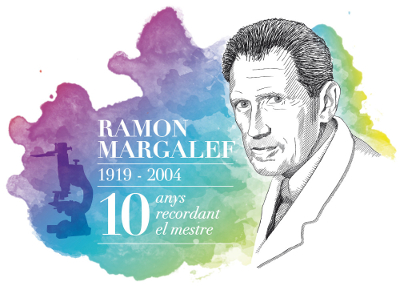
\includegraphics[width=0.8\textwidth]{./figure/logomargalef.png}
    \caption*{textit{Imaxe conmemorativa de actos tralos dez anos da Morte de Ramón Margalef celebrados na \href{www.ub.edu}{Universidade de Barcelona}}}
    \label{fig:icm_memoriam}
\end{figure}

Recibiu multitude de premios científicos, como foron a primeira edición dos \textit{Premios A.G Huntsman para a Excelencia nas Ciencias Mariñas} ou \textit{Medalla de Naumann-Thienemann} e formou parte de sociedades como a \textit{Reial Acadèmia de Ciències i Arts} catalana ou da \textit{Real Academia Galega de Ciencias}.

\subsection{Os seus estudos na Ría de Vigo}
Margalef publicou unha ampla cantidade de estudos da Ría de Vigo: doce publicacións só  década do 1950. Neles describe a composición e variacións nas poboacións de fitoplancto e rotíferos, a dinámica poboacional e as sucesións, a pesquería e a sedimentación, e ata á limnoloxía e paleontoloxía da ría. 

Os estudos máis relevantes describen a composición taxonómica do fitoplancto da ría, o seu ciclo anual e a súa proposta da hipótese da relación entre a turbulencia e a composición taxonómica destas comunidades. O estudo de Margalef \textit{El fitoplancton de la ría de Vigo} (1955) describe por primeira vez o proceso do fenómeno de sucesión nas comunidades fitoplancto en relación con factores ambientais, asentándose nas observacións feitas nas rías galegas. Defíneo como un proceso de tres etapas que abrangue arredor de tres meses, no cal durante a primeira etapa xorden as diatomeas de pequeno tamaño, logo as diatomeas máis grandes e algúns dinoflaxelados e finalmente péchase o ciclo co predominio de dinoflaxelados, dominantes no verán.

No verán do ano 1953 a visita de Margalef á ría, para estudos nesta, coincidiu cunha marea vermella. Grazas a iso, estudou o ata daquela coñecido vulgarmente como a \textit{purga do mar} e publicou os resultados nun artigo do 1956. Incide, iso si, sobre do nome do fenómeno ao mencionar que "...preferimos a denominación hematotalasia introducida por Sobrino (1918), o primero autor español que escribiu sensatamente acerca diso".

Todas as mostraxes dos traballos de Margalef na Ría de Vigo realizounas a bordo da pequena embarcación chamada \textit{Lampadena}. Neses momentos esa embarcación acabara de chegar ao laboratorio de Vigo do Instituto de Investigacións Pesqueiras, e que é o actual \textit{Instituto de Investigacións Mariñas de Vigo}.


\section{Fitoplancto da ría de Vigo, 1951-52}

En \textit{Microplancto de Vigo, de xaneiro do 1951 a setembro do 1952}, Ramon Margalef e Miguel Durán publican un dos primeiros artigos que describen taxonómicamente o fitoplancto da ría e analizan a súa dinámica de cambios na estrutura da comunidade. 

\begin{tabular}{lrrrr}
  \hline
Spp & X & XI & XII & I \\ 
  \hline
Trichodesniium Thiebautii & 0 & 0 & 0 & 0 \\ 
  Dictyocha fibula & 0 & 5 & 5 & 0 \\ 
  Distephanus speculum & 0 & 7 & 9 & 11 \\ 
  Prorocentrum micans & 0 & 11 & 30 & 41 \\ 
  Phalacroma  rotundatum & 0 & 2 & 4 & 11 \\ 
  Dinophysis acuta & 0 & 13 & 30 & 225 \\ 
   \hline
\end{tabular}




Dos $12$ feitos entre o 1951 e 1952 na ría de Vigo, Margalef e compañeiros observaron entre $31$ e $49$ especies de fitoplancto despois de recontar unha media de $69757$ de \href{https://gl.wikipedia.org/wiki/Diatomeas}{diatomeas} e \href{https://gl.wikipedia.org/wiki/Dinoflaxelados}{dinoflaxelados}.
 
Unha representación dos cambios da estrutura da comunidade, dánnola os índices de Shannon e Simpson, que miden canta dominancia ou paridade existe nas comunidades. A definición matemática destes índices é:

\begin{itemize}
  \item índice de Simpson: $ \lambda' = -\sum_{i=1}^S p_i^2 $
  \item índice de Shannon: $ H' = -\sum_{i=1}^S p_i \ln p_i $
\end{itemize}

O mostreo na Ría no que se apreza unha maior dominancia de especies, produciuse no $IX$ mes do 1952.
 
\begin{table}[ht]
\centering
\begin{tabular}{rrrr}
  \hline
 & Species & Simpson & Shannon \\ 
  \hline
X &  31 & 0,49 & 1,23 \\ 
  XI &  47 & 0,84 & 2,43 \\ 
  XII &  39 & 0,85 & 2,35 \\ 
  I &  37 & 0,19 & 0,57 \\ 
  II &  36 & 0,84 & 2,23 \\ 
  III &  44 & 0,80 & 2,34 \\ 
  IV &  46 & 0,90 & 2,67 \\ 
  V &  46 & 0,90 & 2,69 \\ 
  VI &  44 & 0,90 & 2,69 \\ 
  VII &  47 & 0,90 & 2,79 \\ 
  VIII &  49 & 0,89 & 2,72 \\ 
  IX &  33 & 0,92 & 2,79 \\ 
   \hline
\end{tabular}
\caption{Resumo dos índices de diversidade} 
\end{table}

O repetido número de mostreos xa mostra como existe unha cantidade de especies raras, difíciles de obter cunha soa saída de recollida na Ría. Vese por iso como as curvas de acumulación de especies revelan o patrón típico dunha comunidade rica en especies \textit{raras}, ou de baixas abundancias.

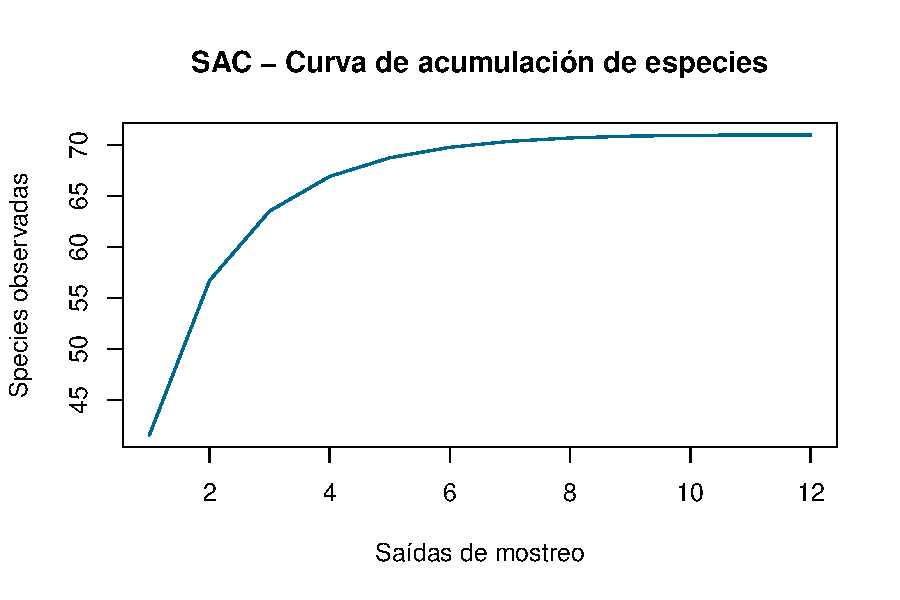
\includegraphics{margalef53-sac}

Un gráfico de Wittaker ou de Rango-Abundancia pon de manifesto como son só unhas poucas especies as que dominan a comunidade fitoplanctónica. 

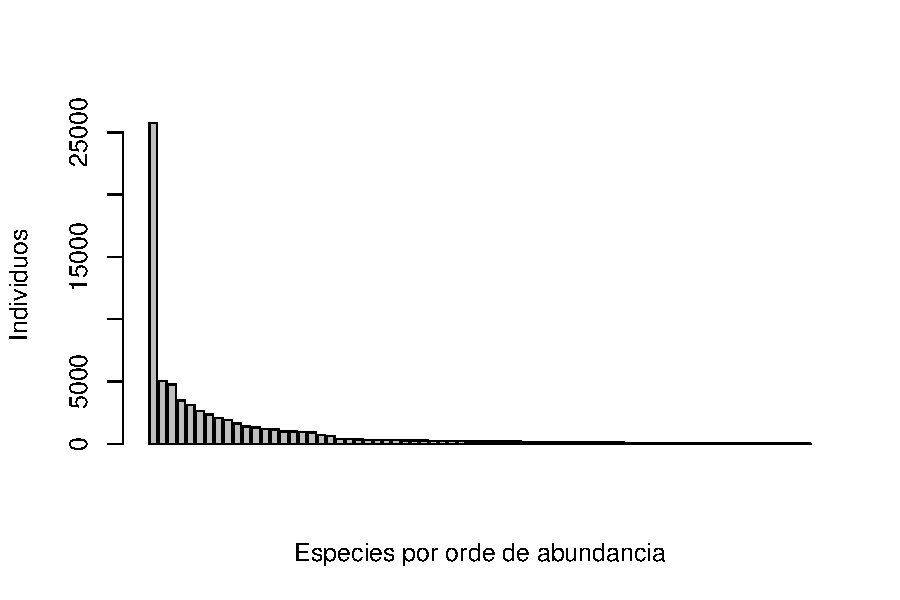
\includegraphics{margalef53-wittaker}

\section{Bibliografía}

\begin{enumerate}
  \item Duran, M., Saiz, F., Lopez-Benito, M., Margalef, R., others, 1956. El fitoplancton de la ria de Vigo, de abril de 1954 a junio de 1955. Invest. Pesq.
  \item Margalef, R., 1956. Estructura y dinamica de la purga de mar en la Ria de Vigo. Inv. Pesq 5.
  \item Margalef, R., Duran, M., Saiz, F., others, 1955. El fitoplancton de la ria de Vigo de enero de 1953 a marzo de 1954. Invest. Pesq.
  \item Nogueira, E., Figueiras, F., 2005. The microplankton succession in the Ria de Vigo revisited: species assemblages and the role of weather-induced, hydrodynamic variability. Journal of Marine Systems 54.
\end{enumerate}

\end{document}
